% Author: Dun-Ming Huang
% Email: dunmingbrandonhuang@berkeley.edu
% CSM16A Fall 2022
%Code references advises on https://tex.stackexchange.com/questions/256863/drawing-and-labeling-angles-in-an-axis-environment

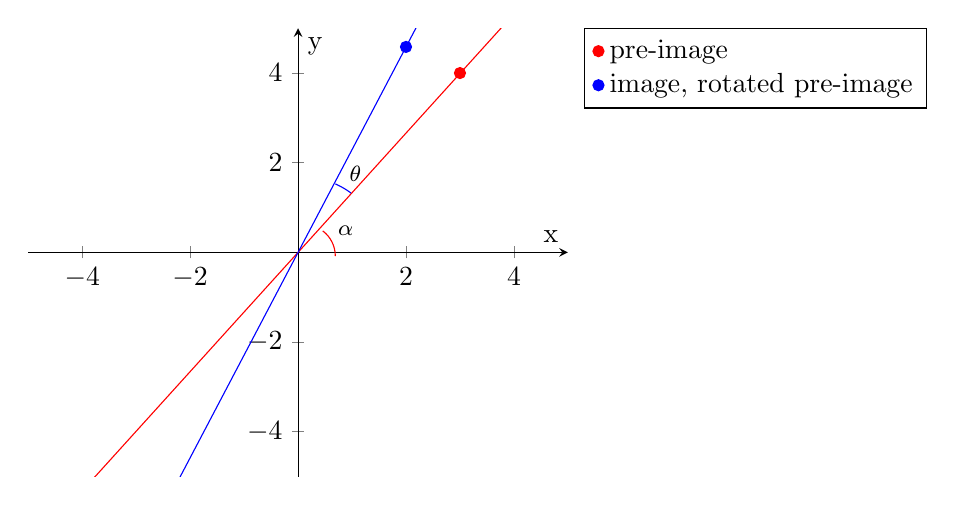
\begin{tikzpicture}
    \begin{axis}[
            axis lines = middle,
            xmin=-5, xmax=5,
            ymin=-5, ymax=5,
            xlabel = {x},
            ylabel = {y},
            legend pos=outer north east,
            legend cell align=left
        ]
        \addplot [only marks, color=red] table {
            3 4
        };
        \addlegendentry{pre-image}
        \addplot [only marks, color=blue] table {
            2 4.583
        };
        \addlegendentry{image, rotated pre-image}
        \addplot [color=red] {
            1.33 * x
        };
        \addplot [color=blue] {
            2.291 * x
        };
        \coordinate (origin) at (0,0);
    \end{axis}
    \begin{scope}[shift={(3.5, 2.8)}]
        \coordinate (O) at (0, 0);
        \coordinate (A) at (3, 4);
        \coordinate (B) at (2, 4.583);
        \draw[draw=blue] (O) ++(53.13:1) arc (53.13:66.42:1)
            node[midway,above right,inner sep=2pt,font={\footnotesize}]{$\theta$};
        \draw[draw=red] (O) ++(53.13:0.4) arc (53.13:0:0.4)
            node[midway,above right,inner sep=2pt,font={\footnotesize}]{$\alpha$};
    \end{scope}
\end{tikzpicture}